% This is samplepaper.tex, a sample chapter demonstrating the
% LLNCS macro package for Springer Computer Science proceedings;
% Version 2.20 of 2017/10/04
%
\documentclass[runningheads]{llncs}

% Packages 
\usepackage{graphicx} % Add assets folder to path for images. 
\graphicspath{{assets/}}
\usepackage{amsmath,amssymb,float,url} % Hide red underlines for URLs. 
\usepackage[hidelinks]{hyperref} % Stack two figures on top of each other.
\usepackage{subcaption} % Make caption text font smaller.
\usepackage{caption}
\captionsetup[figure]{font=small,labelfont=small}
% Make table-caption gap larger (source: https://bit.ly/3zm0wRn)
\captionsetup[table]{skip=10pt}

\usepackage{algorithm}
\usepackage{algpseudocode}

% Used for displaying a sample figure. If possible, figure files should
% be included in EPS format.
%
% If you use the hyperref package, please uncomment the following line
% to display URLs in blue roman font according to Springer's eBook style:
% \renewcommand\UrlFont{\color{blue}\rmfamily}

\begin{document}
%
\title{Fishy Business - Multi-Tree GP Feature Construction for Multi-class Fish Classification}
%
% \titlerunning{Abbreviated paper title}
% If the paper title is too long for the running head, you can set
% an abbreviated paper title here

\author{Jesse Wood\inst{1}\orcidID{0000-0003-3756-2122} \and
  Bach Hoai Nguyen\inst{1}\orcidID{1111-2222-3333-4444} \and
  Bing Xue\inst{1}\orcidID{2222--3333-4444-5555} \and 
  Mengjie Zhang\inst{1}\orcidID{2222--3333-4444-5555} \and 
  Daniel Killeen\inst{2}\orcidID{2222--3333-4444-5555}
}
%
\authorrunning{J. Wood, B. Nguyen, et al.}
% First names are abbreviated in the running head.
% If there are more than two authors, 'et al.' is used.

\institute{Victoria University of Wellington, Te Herenge Waka, PO Box 600, Wellington 6140, New Zealand\\
  \email{ \{jesse.wood, bach.nguyen, bing.xue, mengjie.zhang\}@ecs.vuw.ac.nz}\\
  \and 
  Plant and Food Research, Port Nelson, Nelson 7010, New Zealand\\
  \email{daniel.killeen@plantandfood.co.nz}\\
}

%
\maketitle              % typeset the header of the contribution
%
\begin{abstract}
  % The abstract should briefly summarize the contents of the paper in
  % 150--250 words.
  
  Fish is approximately 40\% edible fillet. 
  The remaining 60\% can be processed into low-value fertilizer or high-value pharmaceutical-grade omega-3 concentrates.
  High-value manufacturing options depend on the composition of the biomass, which varies with fish species, fish tissue and seasonally throughout the year.
  Fatty acid composition, measured by Gas Chromatography, is an important measure of marine biomass quality.
  This technique is accurate and precise, but processing and interpreting the results is time-consuming and requires domain-specific expertise.
  The paper investigates Multi-tree Feature Construction for Multi-Class classification of Gas Chromatography data.
  
  \keywords{
    AI applications \and
    Classification \and
    Feature selection \and 
    High-dimensional data \and
    Multidisciplinary \and 
    Gas Chromatography \and 
    Genetic Program \and 
    Fatty Acid
  }
\end{abstract}

\section{Introduction}

“Kindly let me help you or you will drown said the monkey putting the fish safely up a tree.” -- Alan Watts. 

\begin{itemize}
  \item Wrapper-based Multi-Tree GP for Feature Construction for Multi-class Classification on Gas Chromatography data.
\end{itemize}

\section{Gas Chromatography}

\begin{itemize}
  \item Destructive chemistry technique used to analyze chemical compounds in fish tissue. 
  \item Manual laborious, time-consuming and expensive task. 
  \item Gas chromatograph is intensity vs. time. 
  \item Instrumental drift / alignment issue
\end{itemize}

\section{Preprocessing}

\begin{itemize}
  \item Find missing timestamps.
  \item Impute with zero filling. 
  \item Better classification accuracy for KNN. 
\end{itemize}

\section{Genetic Programming}

Algorithm~\ref{alg:gp} shows the pseudo-code of the GP algorithm used for multiple-feature construction using multi-tree representation to construct $m$ new features, with elitism ratio $e$. 

\begin{algorithm}
\caption{GP-based multiple feature construction}
\label{alg:gp}
\begin{algorithmic}
\State \textbf{Input} : train\_set, $m$;
\State \textbf{Output} : Best set of $m$ constructed features;
\State Initilize a population of GP invidiuals. Each individual is an array of $m$ trees; 
\State best\_inds $\gets$ the best $e$ individuals; 
\While{Maimum generation is not reached} 
  \For{$i = 1$ to Population Size} 
    \State $transf\_train \gets$ Calculate constructed features of individual $i$ on train\_set; 
    \State $fitness \gets$ Apply fitness function on $transf\_train$;
    \State Update best\_inds the best $e$ individuals from elitism and offspring combined;
  \EndFor
  \State Select parent individuals using tournament selection for breeding; 
  \State Create new individuals from selected parents using crossover or mutation; 
  \State Place new individuals into population for next generation; 
\EndWhile
\State Return best individual in best\_inds;
\end{algorithmic}
\end{algorithm}

\section{MCIFC}

A multiple class-independnet feature consturction method (MCIFC) \cite{tran2019genetic}.

\subsection{Representation}

MCIFC is a Multi-tree GP that constructs a smaller number of high-level features, proportional to the number of classes, from the original features. 
This method is based on the intuition that problems with more classes are likely to be more complex, and thus require more features to capture said complexity.
The number of constructed features $m$, determined by $m = r \times c$, where $r$ is the construction ratio (set to 2), and $c$ is the number of classes.
MCIFC constructs 8 features for the 4-class fish species problem and 12 features for the 6-class fish species problem.

\subsection{Crossover and Mutation}

MCIFC limits both the crossover and mutation operators to only one of the constructed features described in Algorithm~\ref{alg:MCIFC}. 
This approach favours exploitation over exploration, making small random changes to constructed features with monotonically increasing fitness due to elitism. 

\begin{algorithm}
\caption{MCIFC Crossover and Mutation.}
\label{alg:MCIFC}
\begin{algorithmic}
\State $prob \gets $ randomly generated probability;
\State $doMutation \gets (prob < mutationRate);$
\If{$doMutation$}
  \State $p \gets$ Randomly select an individual using tournament selection; 
  \State $f \gets$ Randomly select a feature/tree from $m$ trees of individual $p$;
  \State $s \gets$ Randomly select a subtree in $f$; 
  \State Replace $s$ with newly generated subtree; 
  \State Return one new individual; 
\Else 
  \State $p1, p2 \gets $ Randomly select 2 individuals using tournament selection; 
  \State $f1, f2 \gets$ Randomly select a features/trees from $m$ trees of  $p1$ and $p2$, respectively;
  \State Swap $s1$ and $s2$; 
  \State Return two new individuals;
\EndIf
\end{algorithmic}
\end{algorithm}

\subsection{Fitness}

MCIFC takes the balanced classification accuracy of an SVM classifier as the fitness function. 
The SVM classifier is known to be effective for fish oil data \cite{long2022ai}.
Balanced accuracy avoids results bias towards the majority class, which is relevant for the fish species dataset, with the majority class 44\% of samples belonging to fish species blue cod. 
The balanced accuracy is given by 

\begin{align}
  \text{Balanced Accuracy} = \frac{1}{c} \sum_{i=1}^{c} \frac{TP_i}{TP_i + FN_i}
\end{align}

Where $TP_i$ is the number of true positives for class $i$, and $FN_i$ is the number of false negatives for class $i$, c is the number of classes. 

\section{Experimental Setup}

\begin{table}
  \caption{Datasets.}
  \centering 
  \begin{tabular}{ l l l l l }
    \hline 
    Dataset & Features & Instances & Classes & Class Distribution \\ 
    \hline 
    Fish Parts & 4800 & 153 & 4 & 44\% 17\% 20\% 19\% \\ 
    Body Parts & 4800 & 153 & 6 & 15\% 22\% 14\% 22\% 14\% 13\% \\
    \hline 
  \end{tabular}
  \label{tab:datasets}
\end{table}

Table~\ref{tab:datasets} shows the datasets used in the experiments and their respective characteristics.
Due to the high dimensionality of gas chromatography data, this paper employs a GP-based FC approach.
The dataset is suited towards dimensionality reduction, as previous work \cite{long2022ai} demonstrated FS can improve classification accuracy.
The small number of instances is due to the expensive and time-consuming nature of performing Gas Chromatography on fish tissue.

The data is pre-processed to fix the instrumental drift by imputing missing timestamps with zero filling.
Features are normalized in the range [0,1] based on the training set. 

\begin{table}
  \caption{Paramter settings.}
  \centering 
  \begin{tabular}{ l l }
  \hline 
  Function Set & $+,-,*$, neg, protectedDiv \\ 
  Teriminal Set & $x_1, x_2, ..., x_n$, $r \in [-1,1]$ \\
  Maximum Tree Depth & 8 \\ 
  Population size & 100 \\ 
  Initial Population & Half and Half \\ 
  Generations & 300 \\ 
  Crossover & 0.9 \\ 
  Mutation & 0.1 \\ 
  Elitism & 0.1 \\ 
  Selection & Tournament \\ 
  Tournament Size & 3 \\ 
  Construction ratio & 2 \\ 
  % Fitness weighting $\alpha$ 
  \hline 
  \end{tabular}
  \label{tab:parameters}
\end{table}

Table~\ref{tab:parameters} describes the parameter settings of all GP-based methods used in the experiments. 
The function set has standard arithmetic operators ${+,-,\times}$, a protected division operator that prevents division by zero returning 0 instead, and the unary $neg$ operator reverses the sign. 
The feature set, and randomly generated constant $r \in [-1,1]$, are used in the terminal set.
A population of 100 individuals is used for all experiments, with 300 generations.
% A population size is set relative to the number of features in the dataset using coefficients $\beta$ set to 3 for both datasets. 
The construction ratio $r$ used to determine the number of features constructed is experimentally chosen as 2. 
% The fitness weight $\alpha$ is set to 0.8 to bias fitness values towards accuracy. 

\section{Results}

Table~\ref{tab:results} shows the results of the experiments. 
We give the train and test accuracy for the best individual found in the final generation for the fish species dataset. 
The fitness is measures as the balanced classification accuracy on a train-test split of the dataset (66\% train, 33\% test).

\begin{table}
  \caption{Initial Results - Fish Species.}
  \label{tab:results}
  \centering 
  \begin{tabular}{ l l l  }
    \hline
    Method & Train & Test \\ 
    \hline 
    ST & 0.53 & -- \\ 
    MT & 0.55 & -- \\ 
    MCIFC & -- & 0.8673 \\
    SVM & 1.0 & 92.4 \\ 
    \hline 
  \end{tabular}
\end{table}

The table gives results for: 
\begin{enumerate}
  \item ST - Single-Tree GP with classification map \cite{smart2005genetic}
  \item MT - Multi-tree GP with one-vs-rest approach
  \item MCIFC - Multiple Class-Independent Feature Construction \cite{tran2019genetic}
  \item SVM - Linear Support Vector Machine one-vs-rest approach \cite{long2022ai}
\end{enumerate}

\section{Discussion}

The balanced classification accuracy of 86.73\% is a significant improvement on the previous Single-Tree and Multi-tree GP classification, whose best results both could not exceed 55\% accuracy on the training set. Both these approaches fail to capture the complexity of the fish species dataset. For Single-tree GP, this is likely due to the difficulty of the GP finding a single expression that can fit the class boundaires for the classification map. For Mulit-tree GP using the one-vs-rest approach, we see improvement over Single-Tree GP, but still not as good as MCIFC. 

The Multi-tree GP has to learn how to perform accurate classification, which is a difficult task. MCIFC is a wrapper-based method, which plays to the strengths of GP for feature construction, and SVM for classification tasks. 

The Linear SVM classifier has a balanced classification accuracy of 92.4\% on the test set, which is a significant improvement on the previous best result of 86.73\% using MCIFC. However, after tweaking the parameters of MCIFC we expect to match (or exceed) the SVM classifier in the future.

(\emph{Note:} The code needs to be adjusted to record train and test accuracy for each individual to get more comprehensive results, but these initial results were a proof of concept.) 

\section{Conclusion}

\section{Future Work}

Add the Czekanowski distance metric to the fitness function, which puts pressure on the GP to construct features that differentiate effectively between classes in relation to their distance in the feature space \cite{tran2019genetic}. Their paper suggests using an $\alpha = 0.8$ term to bias the fitness function towards accuracy.

Run with the same parameters settings from \cite{tran2019genetic}, a single generation took 1 hour and 28 minutes to evaluate, and with random tree generation, produced the best individual with a test accuracy of 71\%. Compared to an initial fitness of 58\% for the parameter settings given above. It would take 48 hours to evaluate 30 generations, so the results are not included in this paper, but reducing the construction ratio $r$, or population coefficient $\beta$, would significantly reduce this computation. 


% Please note that the first paragraph of a section or subsection is
% not indented. The first paragraph that follows a table, figure,
% equation etc. does not need an indent, either.

% Subsequent paragraphs, however, are indented.

% \subsubsection{Sample Heading (Third Level)} Only two levels of
% headings should be numbered. Lower level headings remain unnumbered;
% they are formatted as run-in headings.

% \paragraph{Sample Heading (Fourth Level)}
% The contribution should contain no more than four levels of
% headings. Table~\ref{tab1} gives a summary of all heading levels.

% \begin{table}
% \caption{Table captions should be placed above the
% tables.}\label{tab1}
% \begin{tabular}{|l|l|l|}
% \hline
% Heading level &  Example & Font size and style\\
% \hline
% Title (centered) &  {\Large\bfseries Lecture Notes} & 14 point, bold\\
% 1st-level heading &  {\large\bfseries 1 Introduction} & 12 point, bold\\
% 2nd-level heading & {\bfseries 2.1 Printing Area} & 10 point, bold\\
% 3rd-level heading & {\bfseries Run-in Heading in Bold.} Text follows & 10 point, bold\\
% 4th-level heading & {\itshape Lowest Level Heading.} Text follows & 10 point, italic\\
% \hline
% \end{tabular}
% \end{table}


% \noindent Displayed equations are centred and set on a separate
% line.
% \begin{equation}
% x + y = z
% \end{equation}
% Please try to avoid rasterized images for line-art diagrams and
% schemas. Whenever possible, use vector graphics instead (see
% Fig.~\ref{fig1}).

% \begin{figure}
% 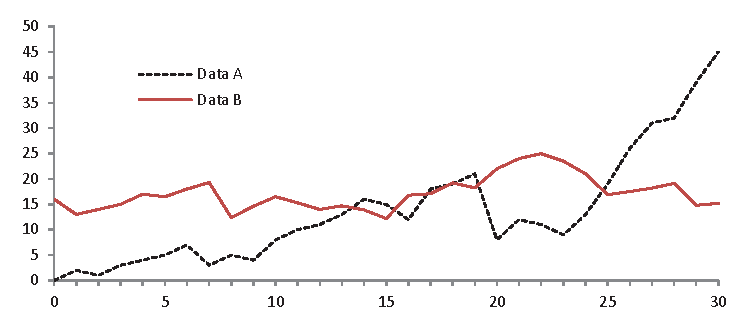
\includegraphics[width=\textwidth]{fig1.eps}
% \caption{A figure caption is always placed below the illustration.
% Please note that short captions are centred, while long ones are
% justified by the macro package automatically.} \label{fig1}
% \end{figure}

% \begin{theorem}
% This is a sampling theorem. The run-in heading is set in bold, while
% the following text appears in italics. Definitions, lemmas,
% propositions, and corollaries are styled the same way.
% \end{theorem}
%
% the environments 'definition', 'lemma', 'proposition', 'corollary',
% 'remark', and 'example' are defined in the LLNCS documentclass as well.
%
% \begin{proof}
% Proofs, examples, and remarks have the initial word in italics,
% while the following text appears in normal font.
% \end{proof}
% For citations of references, we prefer the use of square brackets
% and consecutive numbers. Citations using labels or the author/year
% convention are also acceptable. The following bibliography provides
% a sample reference list with entries for journal
% articles~\cite{ref_article1}, an LNCS chapter~\cite{ref_lncs1}, a
% book~\cite{ref_book1}, proceedings without editors~\cite{ref_proc1},
% and a homepage~\cite{ref_url1}. Multiple citations are grouped
% \cite{ref_article1,ref_lncs1,ref_book1},
% \cite{ref_article1,ref_book1,ref_proc1,ref_url1}.
%
% ---- Bibliography ----
%
% BibTeX users should specify bibliography style 'splncs04'.
% References will then be sorted and formatted in the correct style.
%
\bibliographystyle{splncs04}
% \bibliography{mybibliography}
\bibliography{refs}

\end{document}
